% \documentclass[letterpaper,12pt]{article}
\documentclass[a4paper,10pt]{article}
\usepackage[total={18cm,20cm}, top=1.5cm, left=1.5cm]{geometry}
\usepackage[spanish]{babel}
\usepackage[utf8]{inputenc}
% \usepackage[latin1]{inputenc}
\usepackage[T1]{fontenc}
\usepackage{graphicx}
\usepackage{subfigure}
\usepackage{fancyhdr}
\usepackage{setspace}
\usepackage{hyperref}
\usepackage{multirow}
\usepackage{float}

\renewcommand{\baselinestretch}{1.5}
\pagestyle{fancy}
\rhead{
\includegraphics[width = .055\textwidth]{imagenes/LogoBase.png}}
\lhead{\textit{Social Data Mining \& statistics}}

% \fancyfoot[R]{\includegraphics[width=5mm]{./imagenes/logo.png}}

\title{Comparando tiempos de publicación de redes sociales de automotrices. ¿Cuáles son los mejores días y horas para publicar?}
\author{Social Data Mining \& Statistics \\
        Base10\\
        \scriptsize Dorantes Nieto Fernando ferdorantes@base10.mx \\
        \scriptsize Morán Titla Christian Daniel christian@base10.mx}
% \subtitle{LatReach}
\date{}


\begin{document}

\maketitle

%\begin{abstract}
%\end{abstract}

\section{Introducción}
De los cerca de 7,600 millones de personas que  actualmente viven en la Tierra, cerca
de la mitad (49.3\% ó 3,731,973,423 de personas) usan Internet como medio de comunicación (Internet World Stats, 2017),
el uso de internet incrementa con el paso de los años y de los muchos sitios web existentes
hay algunos cuya popularidad también va en aumento, tal es el caso de las redes sociales,
las cuales son  medios de comunicación que permiten la interacción 
de muchos individuos mediante el uso de la web.\\

Facebook es una de las redes sociales más populares (Smarthinsights, 2016) con cerca de
1,230 millones de usuarios activos diarios (Facebook statistics, 2017).
El propósito de Facebook es el de comunicar  a las personas, sin embargo
su uso va más allá y puede utilizarse con fines académicos o inclusive para el mercadeo (``Marketing'' en inglés) (Wilson et al, 2012).
En el caso concreto del mercadeo, el hecho de que las personas inviertan una buena cantidad de su tiempo en Facebook, 
permite que esta herramienta sea utilizada como un canal de anuncios para diversas marcas (Roshnee y Fowdar, 2013).
La gran cantidad de usuarios con ideas y costumbres diferentes permite a las empresas
realizar diversas estrategias específicas de mercadeo para sus potenciales clientes 
(Casteleyn et al, 2009).\\

El tiempo promedio que una persona pasa en Facebook es de 50 minutos al día (Stewart, 2016),
sin embargo las horas y días en las que una persona pasa en esta red social es diferente
con respecto a la zona geográfica y la ocupación de las personas, por lo que crear estrategias 
para postear (crear contenido en Facebook) también dependerá de estas variables.

En estudios anteriores hechos para el público estadounidense se concluye que el mejor
horario para postear y obtener interacciones es  de 1 a 4 de la tarde en fines de semana, sin embargo, 
si se desea aumentar el número de veces compartido (``shares'') y clicks a las publicaciones de determinada cuenta,
las mejores horas para postear son las 13, 15 y 21 horas (Ellering, 2016), no obstante estos estudios
toman en cuenta solo Estados Unidos por lo que no podrían aplicarse correctamente dichos estudios
al comportamiento de las personas que habitan otros paises.\\

Para el caso concreto de las redes sociales de SEAT y Volkswagen Financial Services
los ``Community managers'' de estas cuentas se esfuerzan en crear estrategias para postear y dar seguimiento a sus clientes,
es por ello que se requiere saber cuales son los mejores días y horas para postear, esta información ayudará a generar mejores estrategias
de mercadeo para sus clientes y fans.\\


Es por ello que el área de ciencia de datos en Base10 propone un experimento
para determinar la mejor hora y el mejor día para realizar posteos y de esta manera
tener una mejor interacción en Facebook con los clientes y fans de SEAT y Volkswagen Financial Services.


\section{Objetivo general}
Determinar la mejor hora y día para postear en Facebook.

\section{Objetivos particulares}
  \begin{itemize}
   \item[$*$] Conocer cual es la  mejor hora para postear en Facebook.
   \item[$*$] Conocer cual es el mejor día para postear en Facebook.
   \item[$*$] Comparar el tipo de contenido (imágenes o videos) que genera mejor interacción en Facebook.
   \item[$*$] Comparar las horas y días de las publicaciones para saber cuál de estas genera una  mayor interacción.
  \end{itemize}


\section{Materiales y métodos}
\subsection{Experimento}
El experimento consiste en obtener el número de posteos diarios de 12 perfiles (Cuadro 1)
públicos de automotrices de Facebook, dichos perfiles deberán ser solo de México, 
la temporalidad de los datos será de  2 años y 4 meses (2015-Abril de 2017).
Para cada perfil, se tomará en cuenta el tipo de posteo, la hora, el día, el mes y año de 
las publicaciones como variables independientes.\\
Las variables de respuesta serán el número de comentarios,
el número de veces compartido y el número de reacciones de cada posteo (Figura 1).
Para el caso de cuentas de Facebook como SEAT y Volkswagen Financial Services, se calculó
el enganche en los periodos de 2016 a Abril de 2017.






\begin{figure}[H]
  \begin{center}
   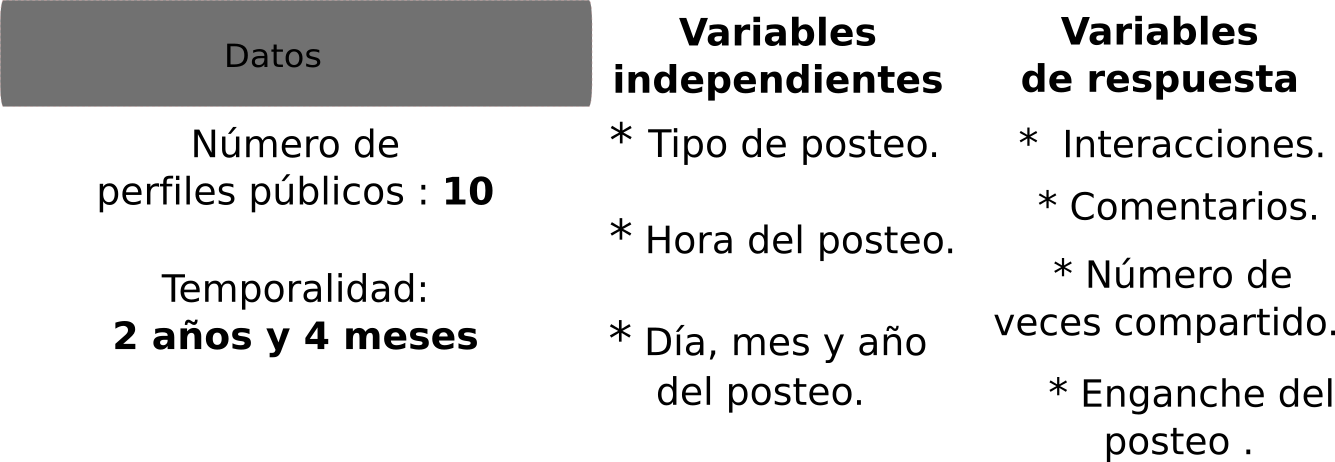
\includegraphics[width=.75\textwidth]{imagenes/figura1.png}
   \caption{Diseño experimental}
  \end{center} 
\end{figure}

\subsection{Recolección de datos}
Los datos de los perfiles de redes sociales se tomarán diréctamente de la API Graph de Facebook 
versión 2.9 (Facebook for developers, 2017), las llamadas a la API se realizaron con el lenguaje de programación Python versión 2.7, 
y el paquete Rfacebook (Barbera et al, 2017) del lenguaje de programación R (R Core Team, 2017)



%\section{Análisis estadísticos}

\begin{thebibliography}{20}
  \bibitem{1} Casteleyn J; Mottart A; Rutten K. (2009). How to use Facebook in you market research. International Journal of Market Research. 51(4) 439-447.
  \bibitem{2} Facebook. (2017). \textit{ Statistics of  Facebook}, Palo  Alto,  CA:  Facebook. Tomado de: http://ltam.newsroom.fb.com/company-info/
  \bibitem{5} Facebook for developers (2017). Tomado de: https://developers.facebook.com/docs/graph-api
  \bibitem{3} Internet World Stats. (2017). Tomado de: http://www.internetworldstats.com/stats.htm
  \bibitem{10} R Core Team (2017). R: A language and environment for statistical computing. R Foundation for Statistical Computing, Vienna, Austria. URL https://www.R-project.org/
  \bibitem{4} Roshnee R; Fowdar S. (2013). The implications of Facebook Marketing for Organizations. Contemporay Management Research. 9 (1) 73-84. doi:10.7903/cmr.9710 
  \bibitem{5} Smarth Insights. (2016). Global social media research summary 2016. Tomado de: http://www.smartinsights.com/social-media-marketing/social-media-strategy/new-global-social-media-research/
  \bibitem{6} Stewart J. (2017). Facebook Has 50 Minutes of Your Time Each Day. It Wants More. Tomado de : https://www.nytimes.com/2016/05/06/business/facebook-bends-the-rules-of-audience-engagement-to-its-advantage.html
 \bibitem{7} Wilson R; Gosling S; Graham L. (2012). A review of Facebook research in the social sciences. Perspectives on Psychological Science 7 (3) 203-220
\end{thebibliography}



\end{document}
